\begin{frame}[fragile]{Relasjoner}
    En relasjon $R$ fra $A$ til $B$ er et subset $ R \subseteq A \times B$. De minner om funksjoner, men er et mer generelt konsept. De er lettere å visualisere ved å tegne dem:
    \begin{figure}
        \centering
        \subfloat{{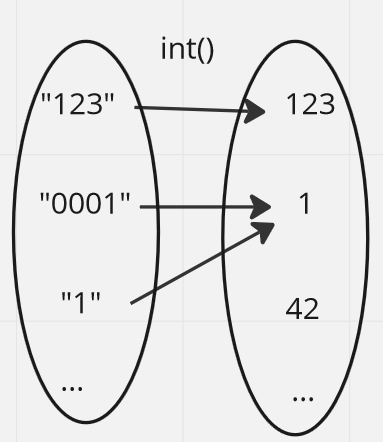
\includegraphics[width=2.8cm]{images/int again.png} }}
        \qquad
        \subfloat{{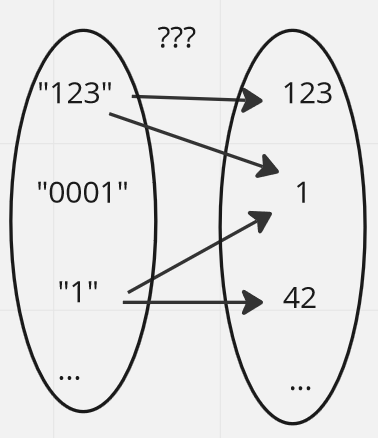
\includegraphics[width=2.8cm]{images/???.png} }}
        \qquad
        \subfloat{{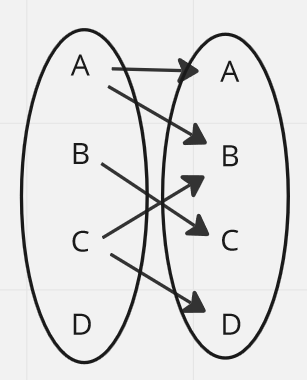
\includegraphics[width=2.8cm]{images/aa.png} }}
        \qquad
        \subfloat{{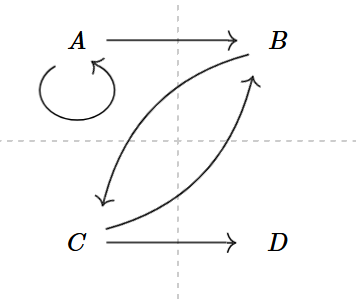
\includegraphics[width=2.8cm]{images/aaa.png} }}
        \label{fig:relasjoner}
    \end{figure} 

    \pause
    Veldig ofte er $A$ og $B$ det samme settet, dvs at $R \subseteq A \times A$.\\ 
    Da kaller vi R en relasjon \emph{på} $A$.
\end{frame}

\begin{frame}[fragile]{Måter å oppgi relasjoner på}
    \begin{columns}
        \begin{column}{0.3\textwidth}
            \begin{tikzcd}
            A \arrow[r] \arrow[d] \arrow[rd] & B \arrow[d] \arrow[ld] \\
            D                                & C \arrow[l]           
            \end{tikzcd}
        \end{column}
        \begin{column}{0.65\textwidth}
            \pause
            Kantliste:\\
            $\{(A, B), (A, C), (A, D), (B, C), (B, D), (C, D)\}$\\[5mm]
            \pause
            Settkomprehensjon:\\
            $\{(x, y) ~ | ~ x, y \in \{A,B,C,D\}, ~ x < y\}$:\\[5mm]
            \pause
            \begin{columns}
                \begin{column}{0.27\textwidth}
                    Matrise:\\
                    \begin{math}
                        \begin{matrix}
                              & A & B & C & D\\
                            A & 0 & 1 & 1 & 1\\
                            B & 0 & 0 & 1 & 1\\
                            C & 0 & 0 & 0 & 1\\
                            D & 0 & 0 & 0 & 0
                        \end{matrix}
                    \end{math}
                \end{column}
                \pause
                \begin{column}{0.38\textwidth}
                    Nabolister:\\        
                    $N(A) = [B, C, D]$\\
                    $N(B) = [C, D]$\\
                    $N(C) = [D]$\\
                    $N(D) = []$
                \end{column} 
                \begin{column}{0.1\textwidth}
                    % padding
                \end{column}
            \end{columns}
        \end{column}
    \end{columns}
\end{frame}




